\documentclass[aspectratio=169,xcolor=table]{beamer}
\usepackage{basileabeam}
\usepackage[ruled,vlined]{algorithm2e}
\usepackage{algorithmic}
\usepackage[english]{babel}

% for colors
\usepackage{xcolor}

% for math formulas
\usepackage{amssymb} % for \mathbb
\usepackage{mathtools} 

% for tables with dashed and dotted lines
\usepackage{tabularray}
\usepackage{booktabs} % For better hlines in tables
\usepackage{multirow}
\usepackage{makecell}

% for images
\usepackage{graphicx}

\setbeamerfont{footnote}{size=\tiny}

% backup slides
\newif\ifincludebackup
%\includebackuptrue  % Uncomment this line to include backup slides
\includebackupfalse   % Comment or uncomment as needed

% Footnote no indention
\addtobeamertemplate{footnote}{\hskip -1.4em}{}

% To includes your notes in the PDF:
%\pgfpagesuselayout{2 on 1}[a4paper,border shrink=5mm]
%\setbeamertemplate{note page}[plain]
%\setbeameroption{show notes on second screen=bottom}

\title              {Trickery with LD\_PRELOAD}

\author             {Project Presentation\\ Carina Fehr, Dehlen Thavarajah, Eda Kaynar, Simon Hammer}

\institute          {Operating Systems Lecture Spring Semester 2025}

\date               {Juni 12, 2025}

\ulogo        		{Template/header}
\ulistelement    	{Template/listelement}

\graphicspath{{./images/}}

% Options:
\totalNoSlidesDisabled % To turn off the total number of slides in the footer. Comment this if you want the total number of slides in the footer
%\headerSectionsDisabled % Comment this if you don't want a fancy header containing your sections.

\begin{document}

% comment this in to generate PDF including notes
%\setbeameroption{show notes}
\setbeamerfont{note page}{size=\tiny}
\setbeamercovered{invisible}
\setbeamercovered{again covered={\opaqueness<1->{100}}}
\renewcommand{\arraystretch}{1.5}

\begin{frame}[t,plain]
\titlepage
\end{frame}

%% to exclude slides from presentation
%\begin{frame}<presentation:0>[noframenumbering]{...}

% ---------------------------------------------------
%\begin{frame}
%\frametitle{Content} 
%\tableofcontents
%\end{frame}

% ----------------------------------------------------

%TODO: 18 min presi, 7 min questions

\section{Slide Section}

\begin{frame}[c]{Problem}
\begin{itemize}
    \item We have a friend who doesn't believe us that we can hack them 
    \item There is no proper Programm to make someone think they got hacked without using 
        code that damages there Software
    \item We want to demonstrate the malicious use of LD\_PRELOAD without harming the OS
    \item This Programm is for pure joy
\end{itemize}

\end{frame}
    \note{
        \begin{itemize}
            \item Your notes if desired. Enabled with uncommenting \verb|\setbeameroption{show notes}|
        \end{itemize}
    }


\begin{frame}[c]{Solution}
\begin{itemize}
    \item We hijacked eight functions that will be loaded in LD\_PRELOAD and then executed 
        before the actually libraries 
    \item Using LD\_PRELOAD we block network connection, changing file access, displaying 
        fake outputs and suppressing command execution. 
    \item We created a bash script to compile and load our hijacked library
    \item Bash script that always loads Hijacked library meaning every new terminal session 
        is affected
\end{itemize}

\end{frame}


\begin{frame}[c]{Hijacked functions}
\begin{itemize}
    \item getchar(): Modifying user input
    \item open(): open another file instead of the one asked for
    \item read(): inject fake data
    \item write(): manipulate terminal output
    \item malloc(): manipulate memory allocations
    \item execve(): execute additional commands 
    \item connect(): restricting network connection
    \item readdir(): modfies ls output,  replacement for getchar
\end{itemize}

\end{frame}

\begin{frame}[c]{Demo}

\end{frame}

\begin{frame}[c]{Timeline}
    \begin{figure}
        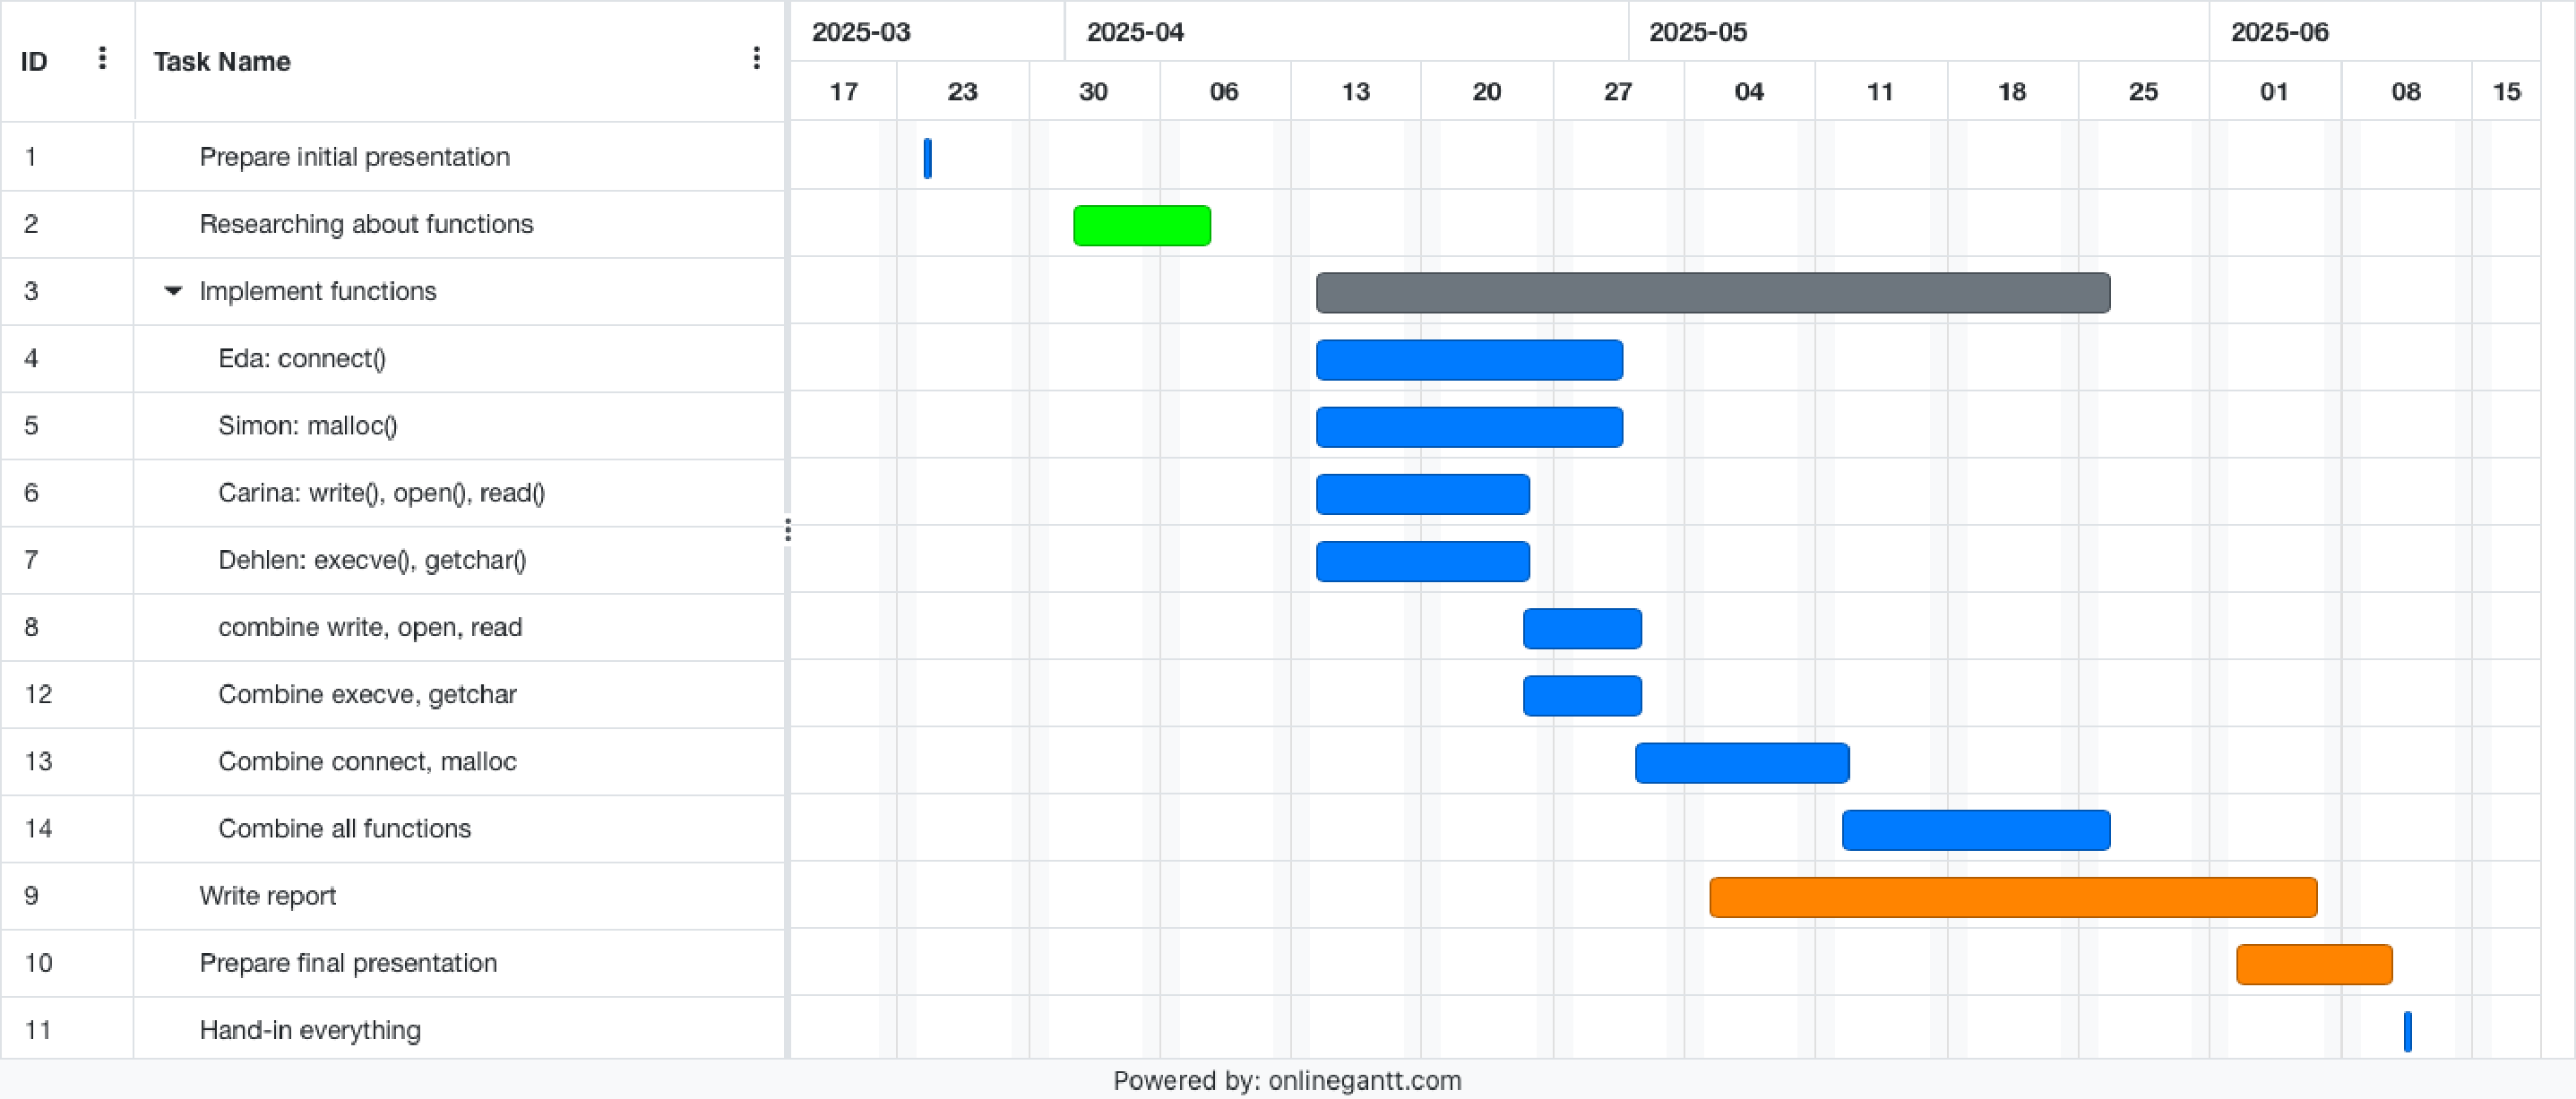
\includegraphics[width=1\textwidth]{images/Online Gantt 20250325.pdf}
        \hfill
    \end{figure}  
\end{frame}

\begin{frame}[c]{Timeline and Discussion}

\begin{itemize}

    \item We distributed the different functions among us. And the report writing as a group 
        task
    \item The combination of the different functions was planed to happen in small steps 
        where the programming person of each function was involved in the Combination 
        with other functions
    \item In the end we didn't have good communication and some people ended up doing 
        more work then others. Some Deadlines where not met which made it hard to 
        finish the hole Library
    \item The Library turned out very nicely. It has a fun touch and plays with fear. 
        Sadly we couldn't make a phishing link or find a way to execute the bash script 
        on its own 
    \item The hardest part was to combine all functions without them interfering each other 

\end{itemize}


\end{frame}
% ----------------------------------------------------



% dont use this for OS, might be used for other lectures: presentation:0
\begin{frame}<presentation:0>[noframenumbering,t,plain]
\lastpage{{\usebeamerfont{title}Questions? Suggestions? Ideas?}\\[5ex]
f.n@mail.com}
\end{frame}


% ------------------------------------------------------
% backup slides
\ifincludebackup

    \begin{frame}[c]{Backup Slides ifdesired
        \begin{itemize}
            \item ...
            \item ...
        \end{itemize}
    \end{frame}    
\fi

\end{document}

    Header \\
    \vspace{10pt}
    \visible<2->{Header second animated slide}
    \vspace{10pt}
    \begin{itemize}
        \item<3-> Itemize on third animated slide.
        \item<4-> Itemize on fourth animated slide.
    \end{itemize}   


    \section{Another section}

\begin{frame}[c]{Another Slide}
    \begin{itemize}
        \item<+> Animated on first click
        \item<+> Animated on second click
    \end{itemize}   
\end{frame}

